\documentclass[12pt]{article}

\usepackage{geometry}
\geometry{margin=1in}
\usepackage{graphicx}
\usepackage[english]{babel}
\usepackage{fancyhdr}
\pagestyle{fancy}
\fancyhf{}
\lhead{Spring 2021 --- PHYS 421 Lab 2}
\rhead{Helen (Yeu) Chen}
\setlength{\parindent}{0cm}
\usepackage{makecell}
\usepackage{amsfonts}
\usepackage{longtable}
\usepackage{amsmath}
\usepackage{amssymb}
\usepackage{amsthm}
\graphicspath{ {./images/} }


\fancyfoot[C]{\thepage}

\begin{document}
\textbf{X-Ray Spectra and Moseley’s Law Experiment}
\bigskip

\textbf{1. \textit{Introduction}}
\smallskip

In this experiment, we analyzed the X ray emission spectra of various elements across a wide range of atomic number $Z$ to determine the screening constant in Moseley's law. Then, we further use the trend we observed for known Z samples to determine the Z values for six unknown samples.

To record the X ray spectrum for each sample we used a XR-100CR semiconductor detector. The incoming X rays is associated with the channel number of the detector according to its energy approximately on a linear scale. Using the Amp-Tek MCA Software, a histogram is generated for each run of measurement with the x axis represents the channel number and the y axis represents the number of times the X-ray with that specific energy is recorded. Then, by carefully identifying the X ray emitted by the sample from the background, the peak location (in terms of channel number) is plotted against Z for all the known sample, and we see all the spectral lines ($K_{\alpha}, K_{\beta}, L_{\alpha}, L_{\beta}$...etc) follow the same relationship (with a different constant C since $\text{channel number} \propto E \propto \frac{1}{\lambda}$) as the Moseley's law:
$$\frac{1}{\lambda} = C(Z- \sigma)^2$$
The screening constant $\sigma$ for each line can be obtained from fitting the known Z data. With this relation in hand, we then identified six unknown sample to be Cr, Ni, Ge, Mo, In, and W.
\bigskip

\textbf{2. \textit{Identifying the unknown samples}}
\smallskip

A major part in identifying the unknown samples is to determine the wether the peak observed is from the K lines or the L lines. To do this, we find patterns between the spectra of the known and unknown samples. The unknowns can be roughly be put into three categories. 

\textbf{I. Fe group:} unknown 1, 2, and 3

In this group, there are two strong peaks in gaussian shape around 1000 similar to Fe, which we know are $K_{\alpha1}$ and $K_{\beta}$ peaks. Below shows a comparison of unknown 1 (Left) and Fe (Right) spectra:

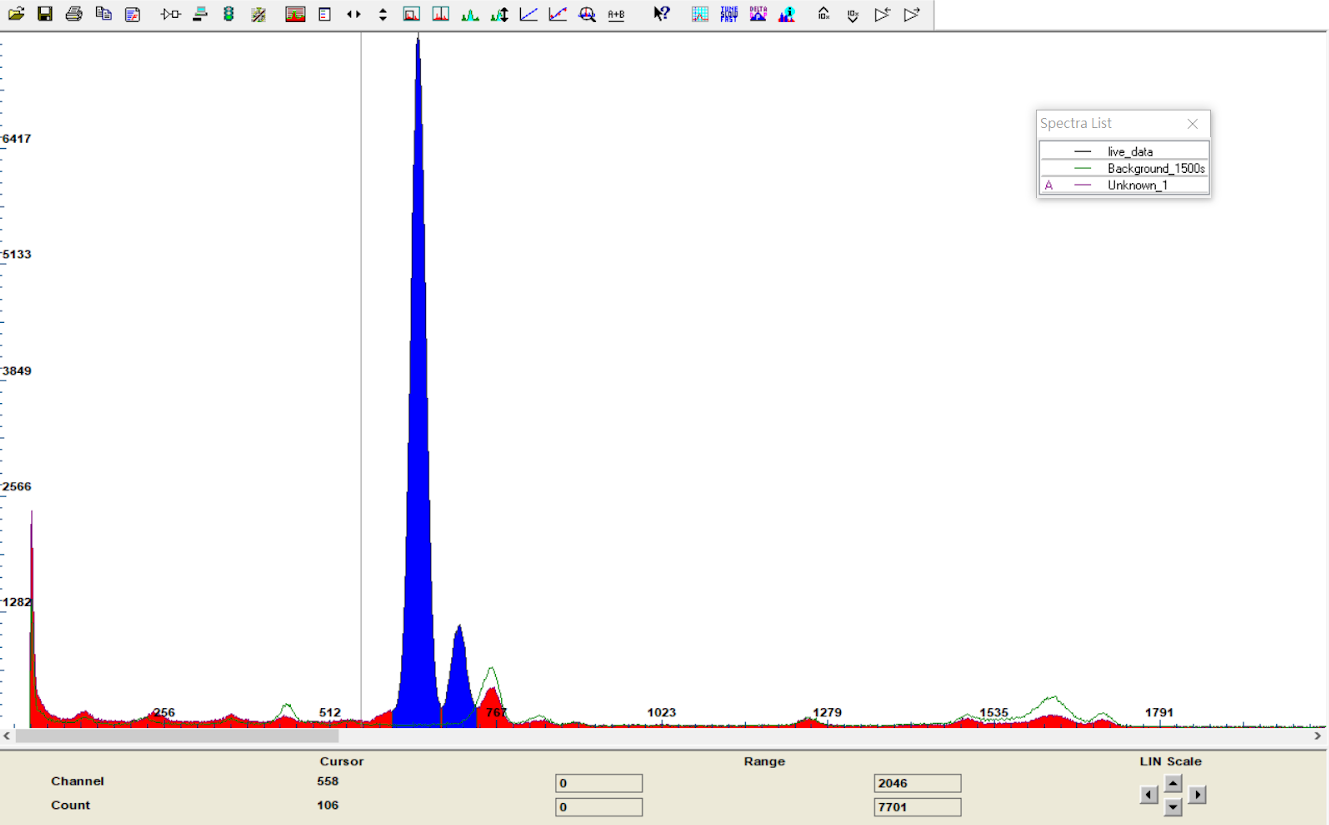
\includegraphics[width=8.5cm]{U1}
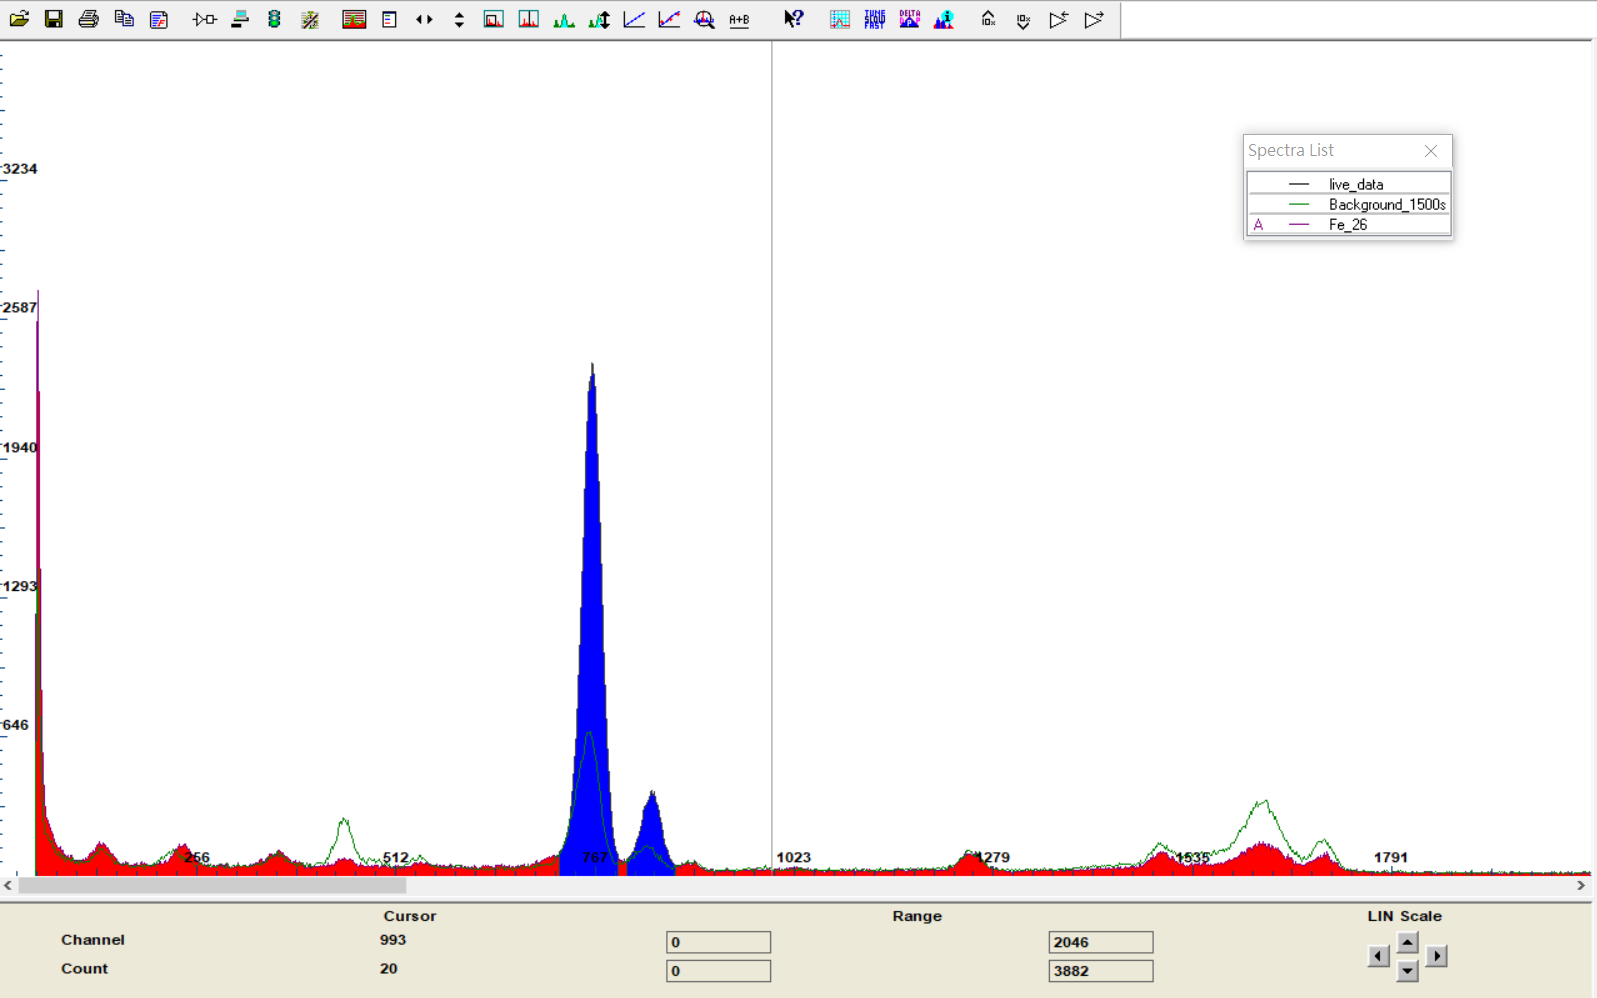
\includegraphics[width=8.5cm]{Fe_26}
\smallskip

\textbf{II. Cd group:} unknown 4 and 5

In this group, there are three gaussian shaped peaks in the 2000 range with smaller intensity. Two are spaced closed to each other with the right one having stronger intensity. This pattern is seen in the spectrum of Cd, and from left to right, the peaks are $K_{\alpha2}, K_{\alpha1}, K_{\beta}$. Below shows a comparison of unknown 4 (Left) and Cd (Right) spectra (notice that the $L_{\alpha}$ is observed in Cd but not unknown 4 since its energy is too low to be seen in later):

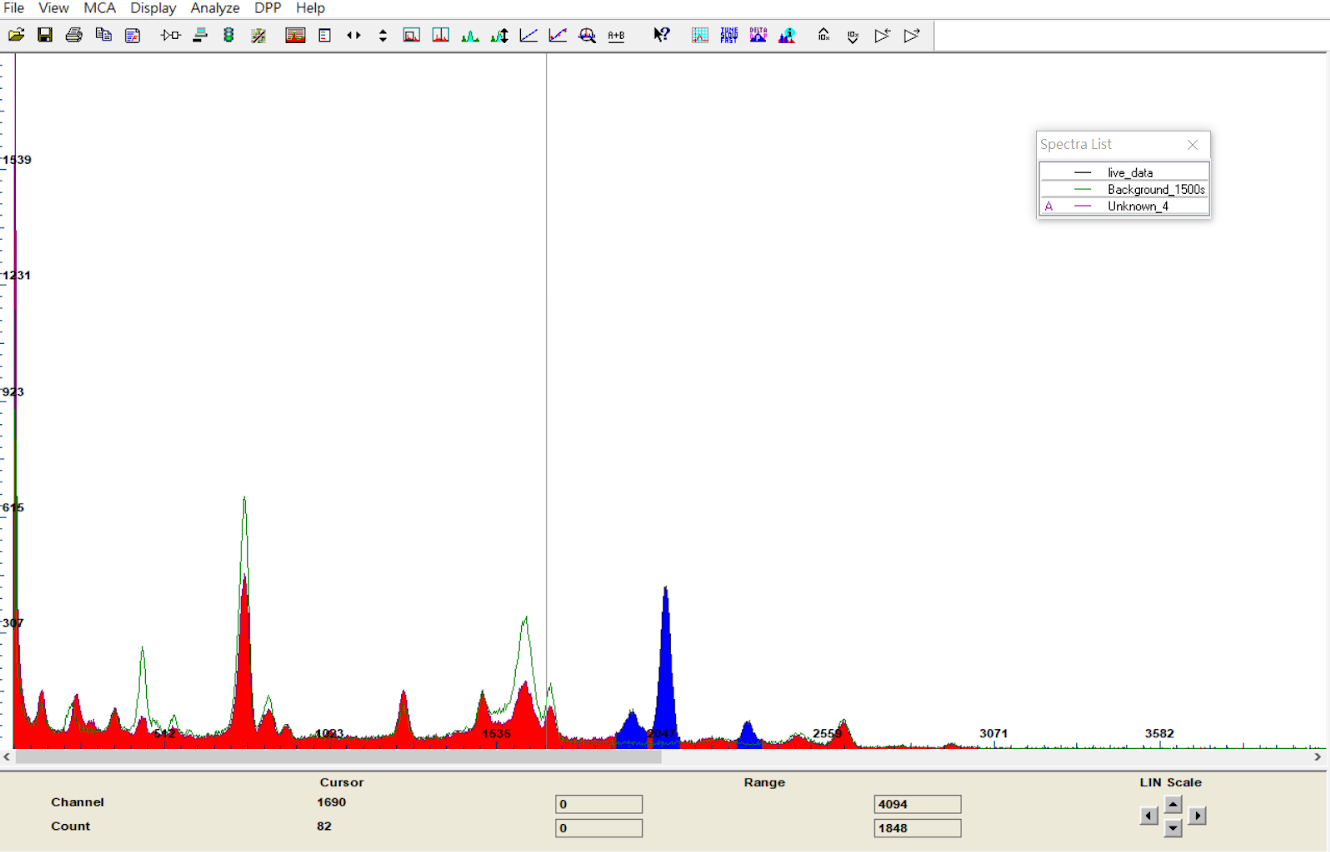
\includegraphics[width=8.5cm]{U4}
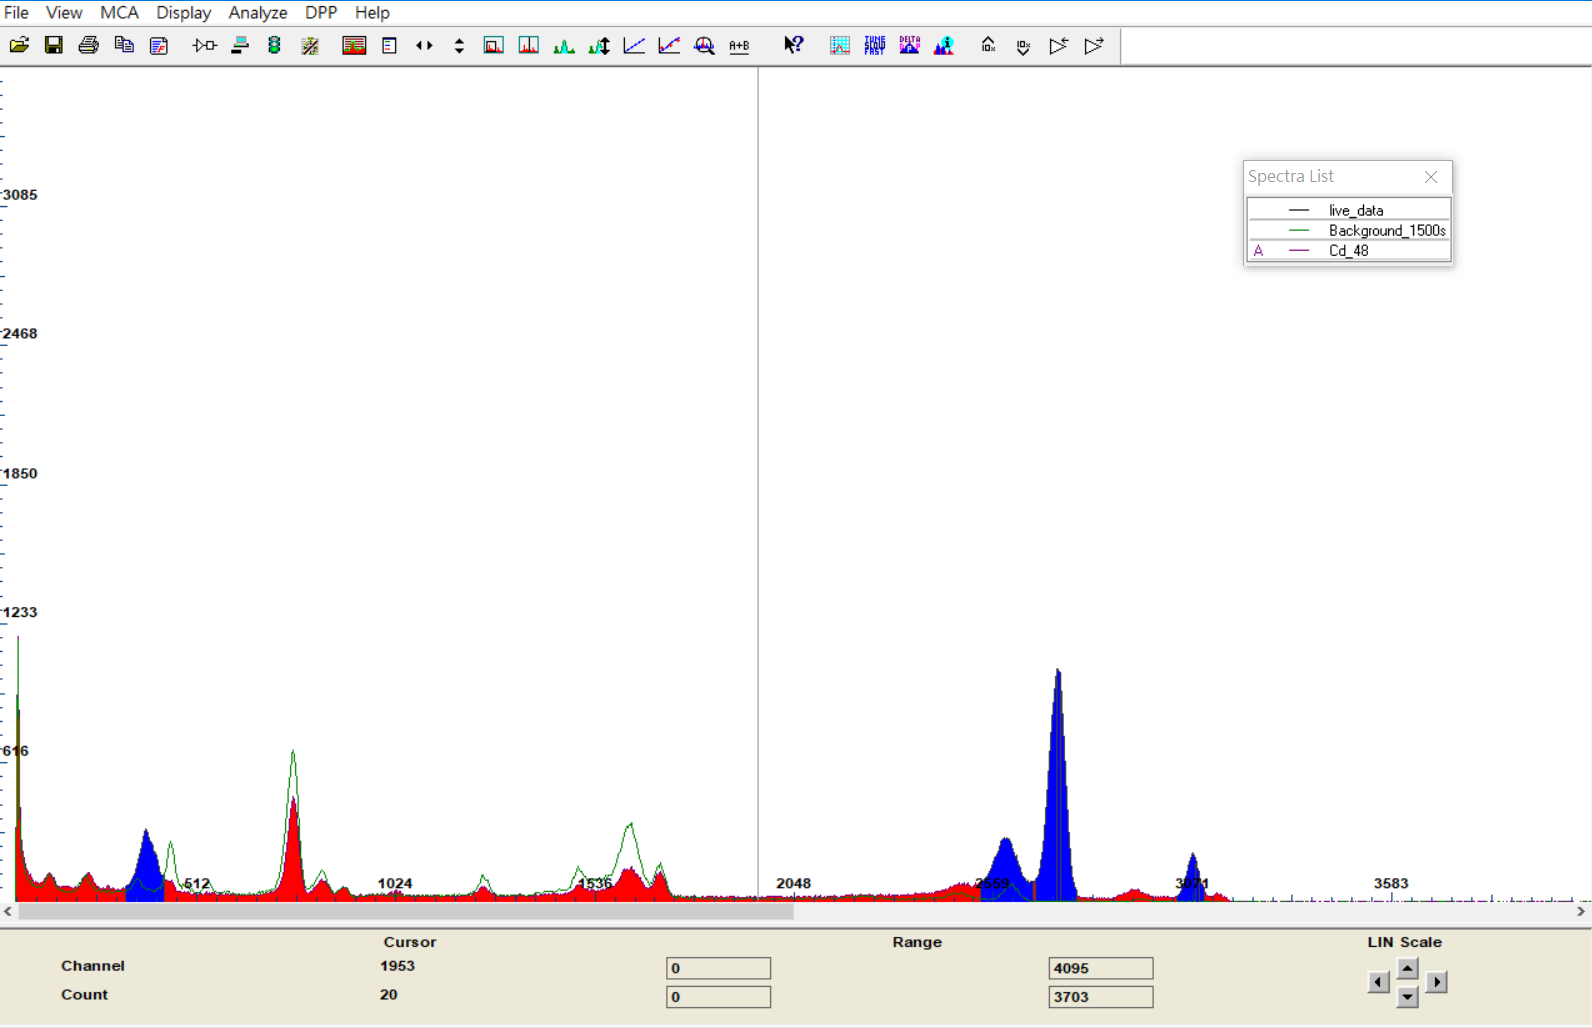
\includegraphics[width=8.5cm]{Cd_48}
\smallskip

\textbf{III. Ta group:} unknown 6

In this group there are two not so symmetric peaks in the 1000 range with strong intensities. Notice their shape is very different from the K lines peaks above. A similar pattern is recorded for Ta, which are, from left to right, $L_{\alpha}$ and $L_{\beta}$ peak. Below shows a comparison of unknown 6 (Left) and Ta (Right) spectra:

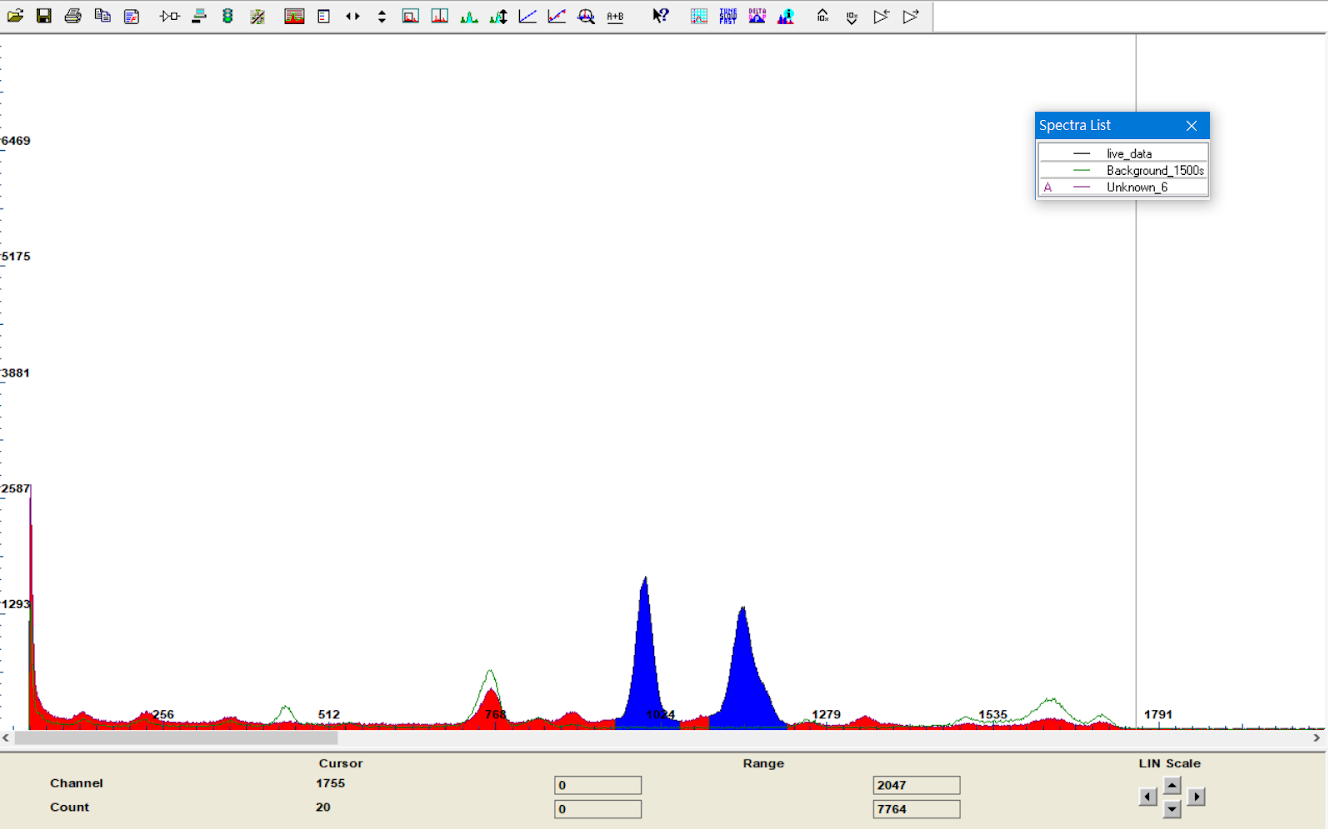
\includegraphics[width=8.5cm]{U6}
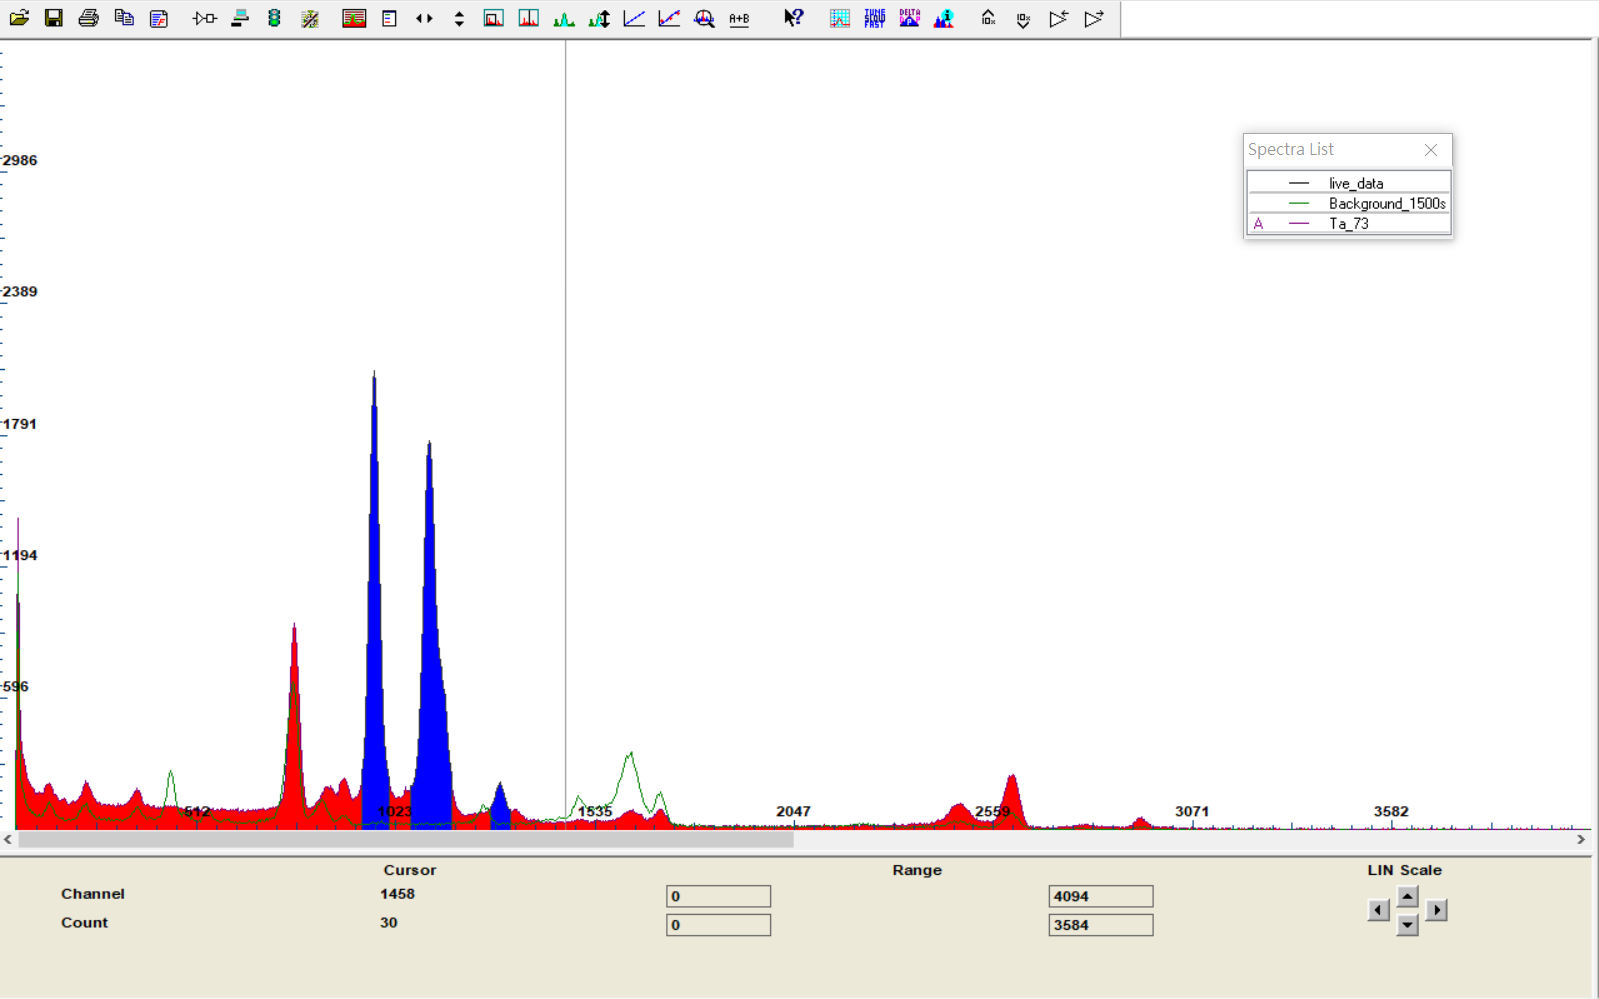
\includegraphics[width=8.5cm]{Ta_73}
\smallskip

Through this process, we have identified which shell transition each peak is belong to for all the unknown, we then can plot the peak locations with the fitted known samples, adjust the unknown's Z such that each peak lies on it's corresponding Moseley line (shown below).
We then found the Z values for unknown 1 to 6 are 24, 28, 32, 42, 49, and 74, which correspond to element Cr, Ni, Ge, Mo, In, and W.

\begin{center}
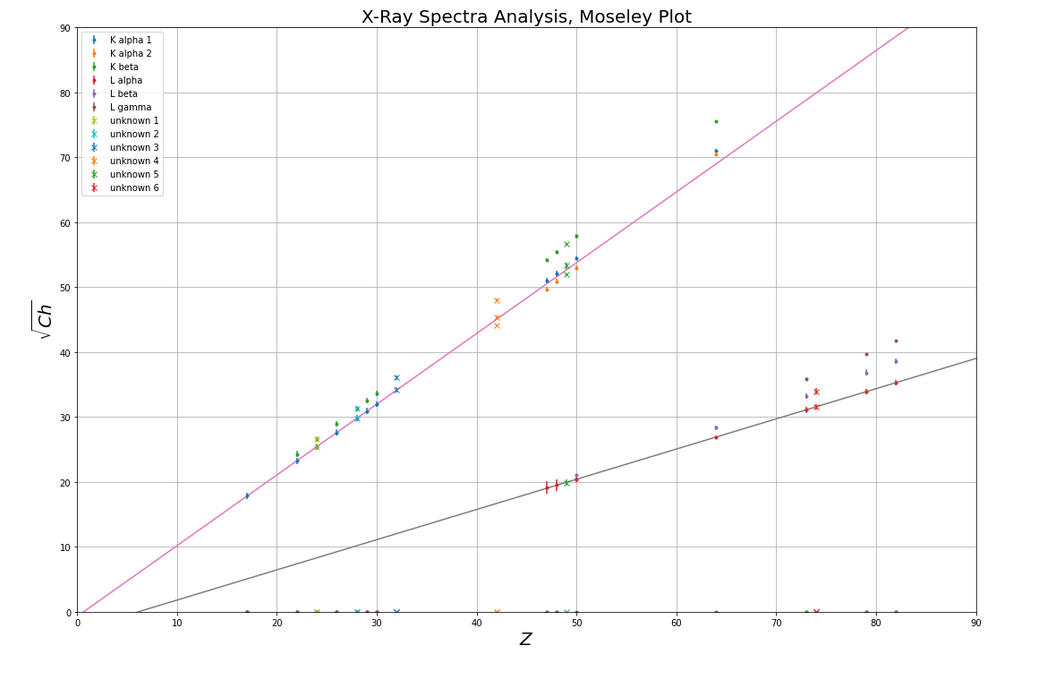
\includegraphics[width=12cm]{unknowns}
\end{center}
\bigskip

\textbf{3. \textit{Aluminum}}
\smallskip

Aluminum has a $K_{\alpha1}$ energy of $1.49keV$ and a $K_{\beta1}$ energy of $1.55keV$. According to the calibration function we obtained from the known samples, they correspond to channel number $186$ and $193$ respectively. In the 120000s background below, we observed no peaks at these location (the vertical line is showing the position of channel 193). For our radioactive gamma ray source (Co 57) the $K_{\alpha1}$ energy is $6.93KeV$, which corresponds to a channel numbers of $823$. As seen from the plot below, we do observed peaks at channel number $831$ (highlighted in blue).

\begin{center}
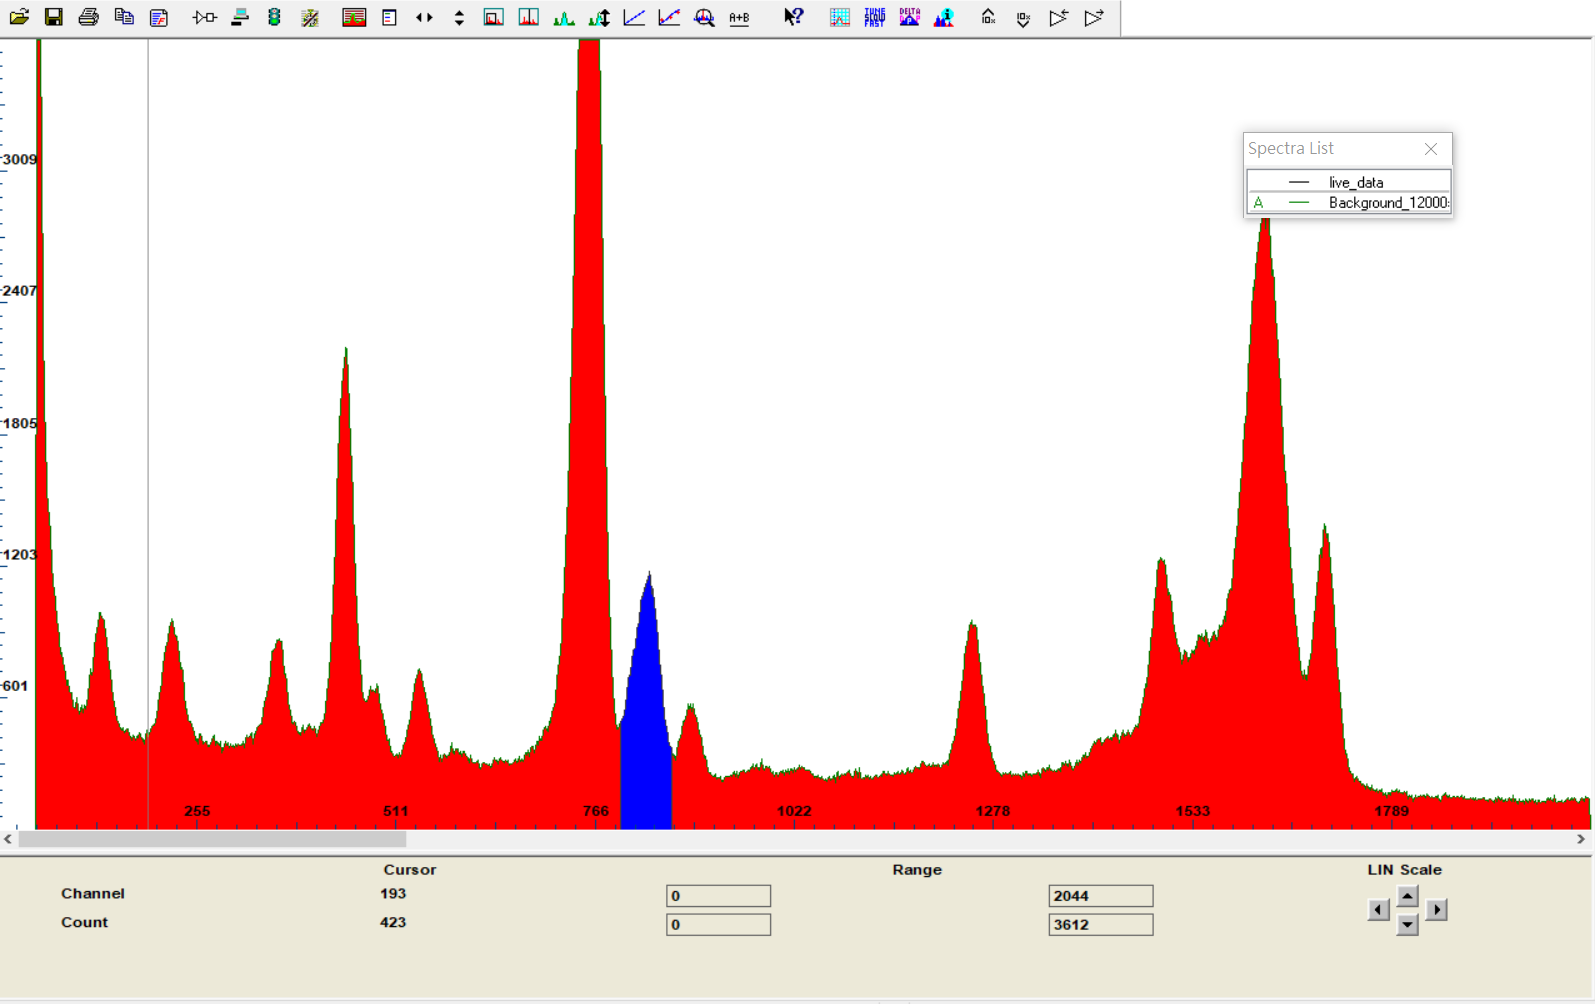
\includegraphics[width=15cm]{background}
\end{center}

\end{document}